\documentclass[10pt,twocolumn,pdftex]{article}
\usepackage[margin=1in]{geometry}
\usepackage{comment}
\usepackage{graphicx}
\usepackage{url}
\usepackage[pdftex,colorlinks=true,citecolor=black,filecolor=black,%
            linkcolor=black,urlcolor=black]{hyperref}
\usepackage{times}

\usepackage{amssymb}
\usepackage{usenix2019_v3}

\usepackage{enumitem}
%----------------------
%extra commands

\usepackage{epsf}
\usepackage{epsfig}
\usepackage{graphicx}
\usepackage{times}
\usepackage{ifthen}
\usepackage{array}
\usepackage{comment}
\usepackage{url}
\usepackage{cellspace}
\usepackage{latexsym}
%\usepackage[margin=1in]{geometry}
\usepackage{amsfonts}
\usepackage{subfigure}
\usepackage{amsmath}
\usepackage{multirow}
\usepackage{multicol}
\usepackage{tabularx}
\usepackage{listings}
\usepackage{amssymb}
\usepackage{mathtools}
\usepackage{wrapfig}
\usepackage{xspace}
\usepackage{enumitem}
\usepackage[compact]{titlesec}
\usepackage{mathpazo,euler}
\usepackage{footnote}
\usepackage{gensymb}
\usepackage{tabularx}
\usepackage{makecell}
\usepackage{pdfpages}
%\usepackage{algorithm}
\usepackage[linesnumbered,ruled]{algorithm2e}
\newboolean{showcomments}

%%%%%%%%%%%%%% PGF Plots
\usepackage[utf8]{inputenc}
\usepackage{tikz}
\usepackage{pgfplots,pgfplotstable}\pgfplotsset{compat=1.9}
\usetikzlibrary{external}
\tikzexternalize[prefix=tikz/]
%%%%%%%%%%%%%% PGF PLOTS

\setboolean{showcomments}{true}

\ifthenelse{\boolean{showcomments}}
  {\newcommand{\nb}[2]{
    \fbox{\bfseries\sffamily\scriptsize#1}
    {\sf\small$\blacktriangleright$\textit{#2}$\blacktriangleleft$}
   }
   \newcommand{\cvsversion}{\emph{\scriptsize$-$Id: macro.tex,v 1.9 2005/12/09 22:38:33 giulio Exp $}}
  }
  {\newcommand{\nb}[2]{}
   \newcommand{\cvsversion}{}
  }
\newcommand\KEVIN[1]{{\color{purple} \nb{KEVIN}{#1}}}
\newcommand\revision[1]{{\color{blue}{#1}}}
\newcommand\ADWAIT[1]{{\color{red} \nb{ADWAIT}{#1}}}
\newcommand\SUNIL[1]{{\color{orange} \nb{SUNIL}{#1}}}
\newcommand\DENYS[1]{{\color{blue} \nb{DENYS}{#1}}}
\newcommand\TONY[1]{{\color{blue} \nb{TONY}{#1}}}
\newcommand\TODO[1]{{\color{red} \nb{TODO}{#1}}}
\newcommand\REF{{\color{blue}[REF]}\xspace}
\newcommand{\tool}{{H$\epsilon$lion}\xspace}
\newcommand{\tools}{{H$\epsilon$lion}'s\xspace}

\newcommand\fix[1]{{\color{blue} \nb{FIX THIS}{#1}}}
\newcommand{\here}{{\color{blue} \nb{***}{CONTINUE HERE}}}
\newcommand{\re}{{\color{red} \textbf{[REFS]}}\xspace}
\newcommand{\xy}{{\color{red} \textbf{XY}}\xspace}

\newcommand{\ie}{\textit{i.e.},\xspace}
\newcommand{\eg}{\textit{e.g.},\xspace}
\newcommand{\etc}{\textit{etc.}\xspace}
\newcommand{\etal}{\textit{et al.}\xspace}
\newcommand{\aka}{\textit{a.k.a.}\xspace}	


\newcommand{\taskref}[1]{{\em Task~{#1}}\xspace}
\newcommand{\rc}[1]{{\bf RC$_{#1}$}\xspace}
\newcommand{\rg}[1]{{\bf RG$_{#1}$}\xspace}
\newcommand{\secref}[1]{Sec.~\ref{#1}\xspace}
\newcommand{\figref}[1]{Fig.~\ref{#1}\xspace}
\newcommand{\tabref}[1]{Table~\ref{#1}\xspace}
\newcommand{\Phase}{{\sc Phase}\xspace}
\newcommand{\Phases}{{\sc Phase's~}\xspace}
\newcommand{\nest}{{NEST}\xspace}
\newcommand{\hue}{{HUE}\xspace}
\newcommand{\smartthings}{{SmartThings}\xspace}
\newcommand{\ngram}{{n-gram}\xspace}
\newcommand{\ngrams}{{n-grams}\xspace}
\newcommand{\seqstart}{{\sf <s>}\xspace}
\newcommand{\seqend}{{\sf </s>}\xspace}
\newcommand{\sequence}[1]{{\em #1}}
\newcommand{\sentence}[1]{\seqstart {\em #1}\seqend}
\newcommand\pnumber[1]{{$\mathcal{P}_{#1}$}}


	\newcommand{\emphquote}[1]{{\emph{`#1'}}\xspace}
	\newcommand{\emphdblquote}[1]{{\emph{``#1''}}\xspace}
	
	\newcommand{\emphbrack}[1]{\emph{[#1]}\xspace}
			
\newcommand{\subj}{\emphbrack{subject}}
	\newcommand{\act}{\emphbrack{action}}
	\newcommand{\obj}{\emphbrack{object}}
	\newcommand{\prep}{\emphbrack{preposition}}
	\newcommand{\objtwo}{\emphbrack{object2}}

	\newcommand*\ciclednum[1]{\raisebox{.5pt}{\textcircled{\raisebox{-.9pt}
	{#1}}}}

\newcommand{\projtodo}[1]{{\color{red}{\bf TODO:}#1}}


\titlespacing{\section}{0pt}{2ex}{1ex}
\titlespacing{\subsection}{0pt}{1ex}{0ex}
\titlespacing{\subsubsection}{0pt}{0.5ex}{0ex}

\newcounter{taskctr}
\newcommand{\task}[1]{
  \addtocounter{taskctr}{1}
  \vspace{0.5em}\noindent{\bf Task \arabic{taskctr}.} ({\it #1})
}

\newcommand{\myparagraph}[1]{\vspace{0.5em}\noindent{\bf #1}:}

\pagestyle{empty}

\definecolor{dkgreen}{rgb}{0,0.6,0}
\definecolor{gray}{rgb}{0.5,0.5,0.5}
\definecolor{mauve}{rgb}{0.58,0,0.82}
\definecolor{shadecolor}{rgb}{0.95,0.95,0.95}
\lstset{ % for our code environment
        language=Java,
        basicstyle=\ttfamily\footnotesize,
        numbers=left,
        numbersep=5pt,
        numberstyle=\tiny,%\color{gray},
        frame=single,
        breaklines=true,
        breakatwhitespace=false,
        breakindent=3pt, % normally 20pt, but need this to be small for now
        captionpos=b,
        %eywordstyle=\bfseries,
        commentstyle=\textit,
        identifierstyle=\ttfamily,
        keywordstyle=\ttfamily
        %stringstyle=\bfseries
}

%----------------------

%remove indentation of itemized/enumeration lists, reduce vertical spacing of bullets
\setlist[itemize]{leftmargin=*, noitemsep, topsep=1pt}
\setlist[enumerate]{leftmargin=*, noitemsep, topsep=1pt}

%spaces before the \paragraph commands
\makeatletter
\renewcommand{\paragraph}{%
	\@startsection{paragraph}{4}%
	{\z@}{0.5ex \@plus 0ex \@minus .2ex}{-1em}%
	{\normalfont\normalsize\bfseries}%
}
\makeatother

%heading spaces
%\usepackage{titlesec} %TODO: move this one to the main file
%\titlespacing\section{0pt}{10pt plus 0pt minus 0pt}{-4pt plus 0pt minus 0pt}
%\titlespacing\subsection{0pt}{10pt plus 2pt minus 0pt}{-5pt plus 0pt minus 0pt}
%\titlespacing\subsubsection{0pt}{3pt plus 0pt minus 5pt}{0pt plus 2pt minus 2pt}

%formula spaces
\makeatletter
\g@addto@macro\normalsize{%
	\setlength\abovedisplayskip{0pt}
	\setlength\belowdisplayskip{0pt}
	\setlength\abovedisplayshortskip{-10pt}
	\setlength\belowdisplayshortskip{0pt}
}
\makeatother

%----------------------

\newcommand*\circled[1]{\tikz[baseline=(char.base)]{
		\node[shape=circle,draw,inner sep=0.5pt] (char) {#1};}}

\DeclareGraphicsExtensions{.pdf,.png}
\graphicspath{{img/}}


%NSF LaTeX Formatting
%%%%%%%%%%%%%%%%%%%%%%%%%%%%%%%%%%%%%%%%%%%%%%%%%%%%%%%%%%%%%%%%%%%%%%%%%
\pagestyle{plain}                                                      %%
%%%%%%%%%% EXACT 1in MARGINS %%%%%%%                                   %%
\setlength{\textwidth}{6.5in}     %%                                   %%
\setlength{\oddsidemargin}{0in}   %% (It is recommended that you       %%
\setlength{\evensidemargin}{0in}  %%  not change these parameters,     %%
%\setlength{\textheight}{8.5in}    %%  at the risk of having your       %%
\setlength{\textheight}{9.1in}    %%  at the risk of having your       %%
\setlength{\topmargin}{0in}       %%  proposal dismissed on the basis  %%
\setlength{\headheight}{0in}      %%  of incorrect formatting!!!)      %%
\setlength{\headsep}{0in}         %%                                   %%
\setlength{\footskip}{.5in}       %%                                   %%
%%%%%%%%%%%%%%%%%%%%%%%%%%%%%%%%%%%%                                   %%
\newcommand{\required}[1]{\section*{\hfil #1\hfil}}                    %%
\renewcommand{\refname}{{\hskip 0pt plus 0.1fil minus 0pt} References Cited\hfil}                   %%
 %%%%%%%%%%%%%%%%%%%%%%%%%%%%%%%%%%%%%%%%%%%%%%%%%%%%%%%%%%%%%%%%%%%%%%%%


%\lstset{ % for our code environment
%    language={},
%    basicstyle=\ttfamily}
%\let\code\lstinline

\title{Leveraging NLP to Enable Analysis of User Driven Routines}
\author{
    {\rm Ruhao (Tony) Tang}\\
    The College of William and Mary\\
    {\rm Department of Computer Science}\\
    {\rm \url{rtang@email.wm.edu}}
}

%-------------------------------------------------------------------------------
\begin{document}
%-------------------------------------------------------------------------------

\maketitle

% Paper Body
%-------------------------------------------------------------------------------
\begin{abstract}

    Routines are trigger-action programs that user create when automating their home. While routine itself offers a wide variety of utilities with a simple conditional format: if \textit{trigger} then \textit{action}, misconfigured or conflicting routines can be potentially dangerous.
    In order to fully analyze home automation, we should not only be required to examine IoT apps, which are routine created by third-party developers, but should also analyze routines from users' perspective, also known as \textit{user driven routine}.
    However, a direct analysis of user driven routines is non-trivial if routines are expressed in natural language, \ie without any constraints on what the user can express. In this paper, we propose an approach that utilize Natural Language Processing (NLP) to automatically transform user driven routines expressed in natural language into intermediate representation, which can later be automatically analyzed. 
    We evaluate this approach with a dataset of 250 user driven routines from a concurrent work. Specifically, we extracted device names (\ie Light Bulb), device capabilities (\ie switch), and device variables (\ie on or off) from user driven routines. This approach produced an accuracy of 80.64\% in one of the intermediate representations transformation. 
These results demonstrated that our approach can efficiently help identifying key device properties from \textit{natural} user driven routines. Furthermore, we separately analyze our intermediate representations to provide additional insights on the characteristic and composition of routines from the end-users' perspective. Finally, we describe some challenges to this approach and propose several potential improvements for future work.
\end{abstract}


\section{Introduction}

% The Introduction includes references to highly-relevant related work,
% i.e., state of the art for the problem you are trying to solve.

% Note: when writing \LaTeX, each paragraph should have a line separated
% between it and the separate paragraph. This causes proper indentation
% and makes the document more readable. Do not end paragraphs with
% \verb/\\/.

%%%%%%%%%%%%%%%%%%%%%%%%%%%%%%%%%%%%%%%%%%%%%%%%%%%%%%%%%%%%%%%%%%%%%%%%%%%%%%%%%%%%%%%%%%%%%%%%%%%%%%%%%%%%%%%%%%%%%%%%%%%%%%%%%%%%%%%%%%%%%%%%%%%%%%%%%%%%%%%%%%%%%%%%

Recent rapid growth of Internet of Things (IoT) technology has made home automation more attractive and more affordable. With smart home devices becoming increasingly more popular, over 20 billion of them are projected to be in use by 2020,~\cite{iot-adoption} numerous smart-home platforms start to appear on the market. Much of the rise in popularity can be attributed to the tremendous utility offered by the smart devices, in which they were able to offer the convenience of automating their home. These devices range from small motion sensors to large digital house appliances such as refrigerator, and enable complex operations across devices (\eg "Turn on the security camera when a motion is detected while I am away from the house"). However, with increasing in convenience of home automation, the associated security risk is also increasing. In addition, automation of smart home opens the attack surface of cyber-physical environment, allowing adversaries to compromise and endanger users' safety without physical access to users' residence. For instance, an adversary can exploit a SSL vulnerability to compromise a door lock, and with that, gaining physical access to a place that is not normally accessible. Just recently, by exploiting the use of common factory default username and password in over 600,000 IoT devices, a historically large scale Distributed Denial of Service (DDoS) attack was launched by Mirai Malware trying to cause a massive Internet shortage.~\cite{tzl+17}

%With increasingly more smart devices coming into consumers' lives, many cloud connected smart devices such as thermostats, security cameras, and smart door locks are being deployed by homeowners. One recent study has predicted that home automation will generate more than \$100 billion in revenue, drawing even more vendors into this ever growing industry.\TONY{Citation here, Tian 2.1}. These new platforms are bringing in more innovating ideas to manages these smart devices. One such example would be Samsung's' SmartThings, which allows smart devices to be connected with a cloud-connected smart hub. Similar vendors typically host third-party IoT apps on their servers, which adds the feature of remote monitoring and controlling to user's home. Most IoT apps can get access to the status of sensors.

%Most Smart home platforms such as Samsung's SmartThings, Google's NEST, and Apple's HomeKit enable home automation through a series of \textit{routines}, trigger-action programs. In essence, these individual trigger-action programs forms the basic building block of complete home automation. Users can specify any \textit{action} events to execute whenever a specific \textit{trigger} condition is satisfied. For example, whenever the user leaves the house (\ie trigger), turn the security camera ON (\ie action).  Previously research has analyzed routines to identify unexpected consequence of home automation and track private data leak. These inspiration often are drawn from the rich domain of Android Security Research. While such an approach may have its advantages (\eg allowing re-use of existing tools and techniques), it has has a critical negative side effect: prior researches generally focus on IoT apps that are build by platform or third-party developers on the public marketplace (\eg SmartApps from the SmartThings marketplace). By focusing only on this specific part of the problem, the prior research fails to account and address the area from the user's side, \ie routines created by end-users.  

End-user programming is often done via a trigger-action framework provided by most Smart Home platforms. These platform vendors often provide an interactive user interface (UIs) that allows user to configure and customize their individual routines. Such design is in a stark contrast to application based platform like Android or iOS, where users depend entirely on applications build by third-party developers. These UIs allow users to create routines by tying together the capabilities of individual devices in the form of trigger-action chains, allowing users who do not have any programming experience to create such programs with ease. However, these user-driven home automations can be problematic since it introduces a set of unexplored scope that may not be apparent from just analyzing IoT apps built by platform vendors or third-party developers. This is illustrated by the dataset we used from a concurrent work which collected from the Computer Science department, in which 107 out of 250, 42.8\%, routines created by 37 users cannot be represented by any of the IoT apps offered by the public SmartThings market. This perfectly demonstrates the existence of a mismatch between user needs and developer-provided functionalities. In addition, this mismatch highlights the unknown nature of user-driven routines and complicates the practical security analysis.

By enabling consumers to control and automate a diverse set of physical objects in their home, home automation platforms are offering a new level of functionality and convenience. While this convenience can be advantageous and beneficial, security flaws in the platform or any smart device can have severe consequences for the safety of users' physical environment. Prior work by Kafle et al.~\cite{kmm+19} has demonstrate the potential for the misuse of routines in Google's NEST platform by being able to perform a lateral privilege escalation attack. During this attack, they were able to first compromise a third-party app that only had access to a low-integrity device (\eg TP Link Kasa Switch), and using the compromised app to trigger an execution of a security sensitive routine, thereby \textit{indirectly} change the state of a high-integrity device (\eg the NEST security camera).This finding motivates the need to assess the security of home automation using a holistic approach.
Similarly, Celik et al.~\cite{cmt18} proposed a static analysis system, Soteria, that can detect side-effects of concurrent execution of IoT apps. Soteria demonstrated that some IoT apps may accidentally trigger an execution of another app, thus leading unexpected and often harmful side-effects. In a similar fashion, IoTMon~\cite{dh18} has demonstrated how malicious applications could deliberately affect environment factors such as the temperature in order to trigger other IoT app. 

Many similar prior works have addressed many IoT security problems by demonstrating the potential benefits to analyze not just IoT apps but also the execution of them. While the lessons and insights from prior work are valuable, they all suffer one common critical limitation: \textit{one-sided perspective}. By analyzing solely on IoT apps from either platform vendors or third-party developers, prior work limited their analysis by relying on a potentially narrow and limited developer's perspective. Although this focus is certainly important, limiting focus to developer's perspective will undoubtedly prevent stakeholders prioritizing more realistic problems that can occur in home automation setup. This limitation motivates the main contribution of the paper, a method that enables analysis of user-driven routine to facilitate a natural perspective of home automation.


As mentioned previously, most prior work that assess the security of home automation draws insight from analyses of IoT apps, but the nature of such analyses is limited and can only be applied to existing routines that they are analyzing.
To overcome this limitation, we have to examine user-driven routines. However, analyzing user-driven poses several challenges: {\sf (1)} data collection of user-driven routines; {\sf (2)} develop a systematic approach to analyze \textit{natural} language. We were able to overcome the first challenge with a dataset of 250 routines from a concurrent study and propose a systematic approach that leverages NLP tools and techniques to transform user-driven routines into meaningful intermediate representation.


%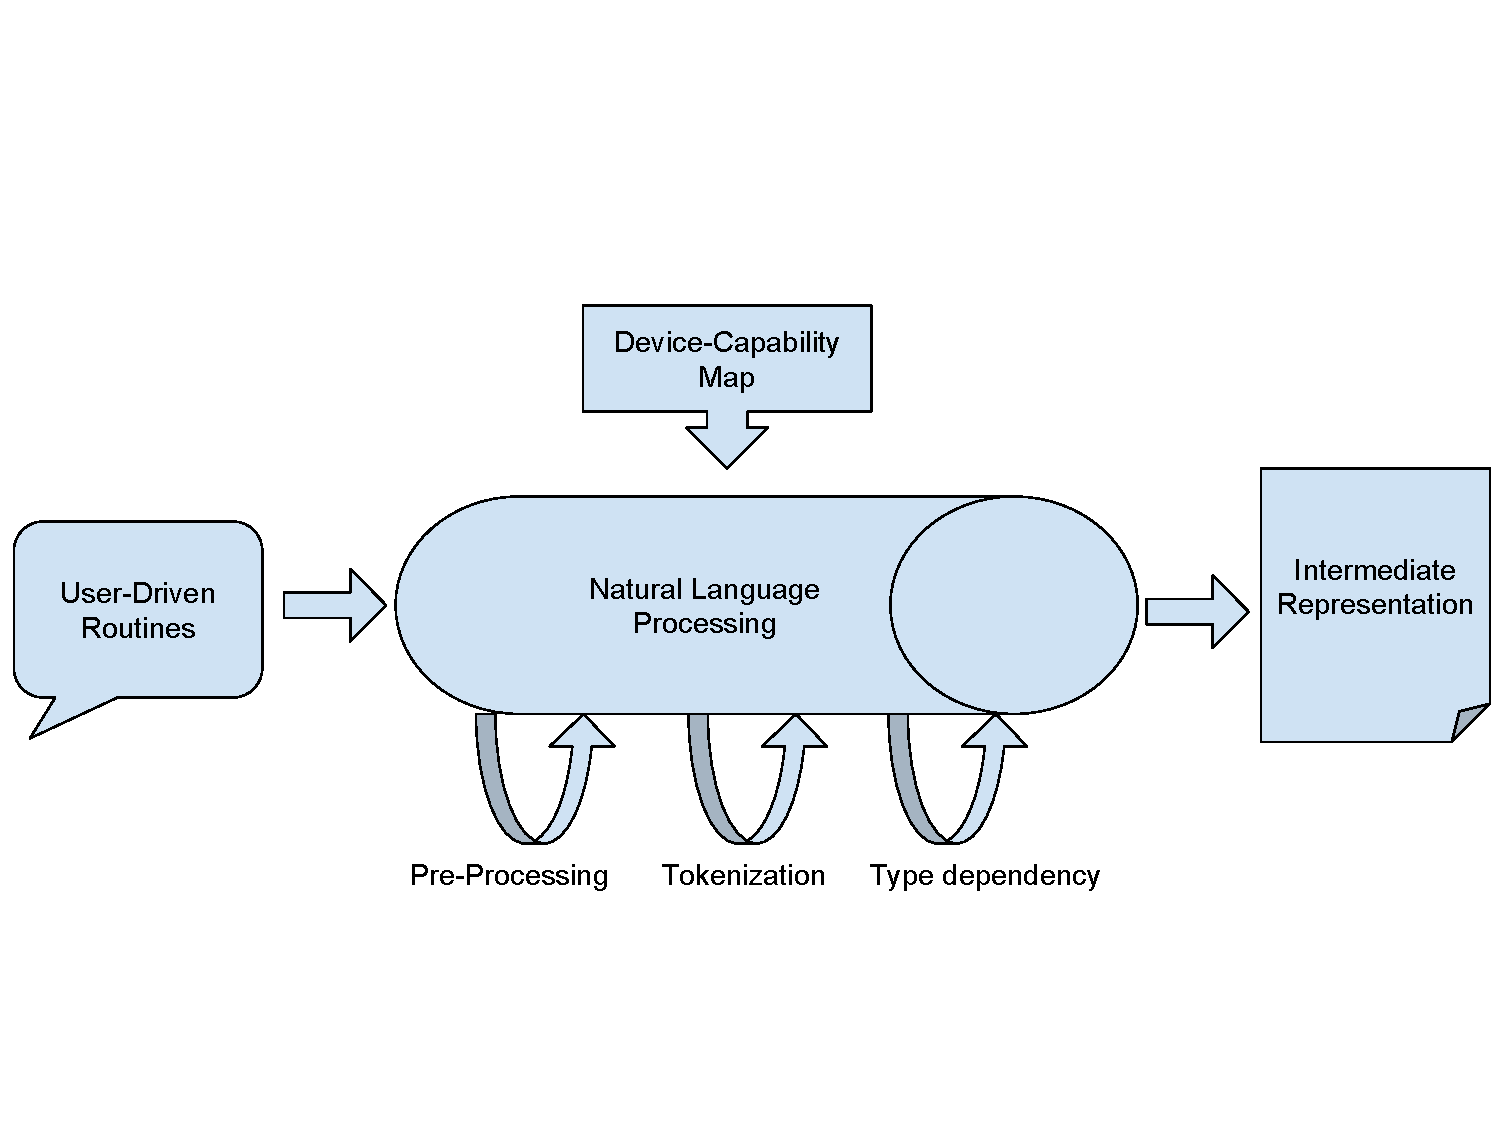
\includepdf[scale=0.5]{figs/nlp-tool.pdf}
The contributions of this paper are as follows:
\begin{itemize}
    \item We motivate the need for a holistic evaluation of home automation through the analysis of {\em user-driven routines}
    \item We develop a systematic approach that enables analysis of user-drive routines by converting them into intermediate representation. 
    \item We analyze the result of these intermediate representation and provide insights to a series of question regarding the characteristics and compositions of user-drive routines.
\end{itemize}


The remainder of this paper proceeds as follows:
In Section~\ref{sec:background}, we provide some background information on the dataset that we are using and the reason behind it.
In Section~\ref{sec:motivation}, we describe the motivation behind the transformation of user-driven routines to intermediate representation using NLP.
In Section~\ref{sec:design}, we describe the high-level design and details on each stages of our proposed approach, and our evaluation of these models follows in Section~\ref{sec:eval}. 
Section~\ref{sec:insight} provides additional insights from the generated intermediate representations.
Section~\ref{sec:discussion} discusses the limitation of the models and possible improvement for future work.
In Section~\ref{sec:related-work}, we highlight relevant related work, and 
Section~\ref{sec:conc} concludes.

\section{Background}
\label{sec:background}

%% Home automation security
% 
%This paper is motivated by a gap in the domain of home automation security, and resolves the gap using an approach inspired by prior treatment of software as a natural language.
%This section attempts to address related work in both these domains. 

%\myparagraph{1. Home automation security}
One of the main challenges of analyzing user-driven routines is obtaining them from existing or potential users. To achieve this, we utilize an existing dataset of 250 user-driven routines collected from a concurrent work. Participants were given the option to select any number of smart home devices from a list of 70 for their ideal smart home setup. In addition of receiving a device list, participants were provided with a device-capability list to guide with the creation of routines. Most importantly, participants were able to create routines for their smart home in the form of plain English text, which overcomes the first challenge for this study (\ie data collection of user-driven routines).
% ========== NLP TECHNOLOGIES ========== 
\subsection{NLP Tools and Techniques}

While the routine from our dataset is in a semi-structured format, parsing each one is still a non-trivial task. To analyze these phases, we rely on several existing natural language processing (NLP) tools and techniques.
The first tool we tried to employ was NLTK, a Natural Language Toolkit written in Python ~\cite{nltk}. NLTK is a leading platform for building Python programs to work with data related to human languages. In addition to have more than 50 corpora such as WordNet, NLTK also provides a suite of libraries for stemming, tagging, tokenization, semantic reasoning, and pre-processing.

It turns out that NLTK is excellent for pre-processing and tokenizing natural text, however, it is still lacking in correctly identifying the part of speech (POS) of each word.
Part-of-Speech tagging is used to identify a word's part of speech based on its context and definition.  For instance, the NLTK POS tagger tagged ``thermostat'' as a ``JJ'' (Adjective). This is problematic since ``thermostat'' is device that is quite commonly used as a device. This prompted the need to search for an alternative tool to perform POS Tagging.

Stanford CoreNLP, on the other hand, provides a more comprehensive library that does not only have a higher accuracy in POS tagging than NLTK, but also allows the parsing of syntactic dependencies of each word. This is particularly useful in that it helps us understand the grammatical structure of each sentence, and it is able to recognize different phases within a complex routine and pair subjects or objects with respect to the associated verb.



\section{Motivation}
\label{sec:motivation}

\begin{table*}[t]
\centering
\scriptsize
\caption{{\small Examples of complex routine created by users.}}
\label{tbl:complex-routines}
\begin{tabular}{l|l}
\Xhline{2\arrayrulewidth}
{\bf No.}& {\bf Trigger}\\
\Xhline{2\arrayrulewidth}
1 & (The presence sensor is not detected for more than 1 hour OR the time is between 1AM and 5:30AM) AND the door is unlocked \\
2 & The blinds are closed AND the time is between 10AM and 6PM AND the motion sensor does not detect motion\\
3 & The mode is Vacation AND Gas Sensor odorLevel reach "X" OR Water Leak Detector is wet OR carbonMonoxide Level is above "Y"\\
\Xhline{2\arrayrulewidth}
\end{tabular}
\end{table*}



In order to obtain unconstrained user-driven routines from users, participants provided routine in plain English text. While this approach provides maximum flexibility and reflects \textit{direct} users' requirements, there are several complications that make \textit{automatic} analysis of user-driven routines a non-trivial task.
We can summarize the complications as the follows:
\begin{itemize}
    \item \textbf{Complication 1:} Many desired behaviors for one smart home automation can involve more than one smart device. Specifically, some trigger or action or a combination of both might can incorporate multiple devices.

    \item \textbf{Complication 2:} In practice, users often combine multiple triggers in a large number of unique ways. For example, user can specify to turn off the security camera when user is at home AND it is morning. 

    \item \textbf{Complication 3:} Since routines are written in plain text, key device attributes and state variables are often \textit{implicit}. For example, one user created the following routine: If the temperature is low, then change the thermostat mode to cold. In this case, there is no references of a device name in the trigger part of the routine. 
\end{itemize}

\subsection{Motivating Examples}
We introduce three noticeable samples of user-driven triggers for exposition and illustration (Table.~\ref{tbl:complex-routines}). Each of these routines demonstrated one or more complications describe above. For example, the first user-driven trigger is:
\noindent\fbox{%
    \parbox{\linewidth}{%
(The presence sensor is not detected for more than 1 hour OR the time is between 1AM and 5:30AM) AND the door is unlocked.
	}
}

To begin, this trigger requires multiple devices (Challenge 1) separated by conjunction ``AND'' and ``OR''. In addition, although the fact that the trigger ``door is unlocked'' is referring to door lock is obvious to us, a traditional script will not be able to recognize it since smart door does not 'exist', and the only commercially available parts relating to door are door lock, or doorbell. 

Based on these observations, a general static analysis script without using NLP would not be \textit{effective} in automatically gather and output the desired intermediate representations of user-driven routines. Therefore, we propose the following framework that leverages state-of-art NLP toolkits and techniques to perform the transformation of user-driven routine to intermediate representations. (Figure.~\ref{fig:nlp-framework})


\section{Design and Implementation}
\label{sec:design}


\begin{figure*}[t]
    %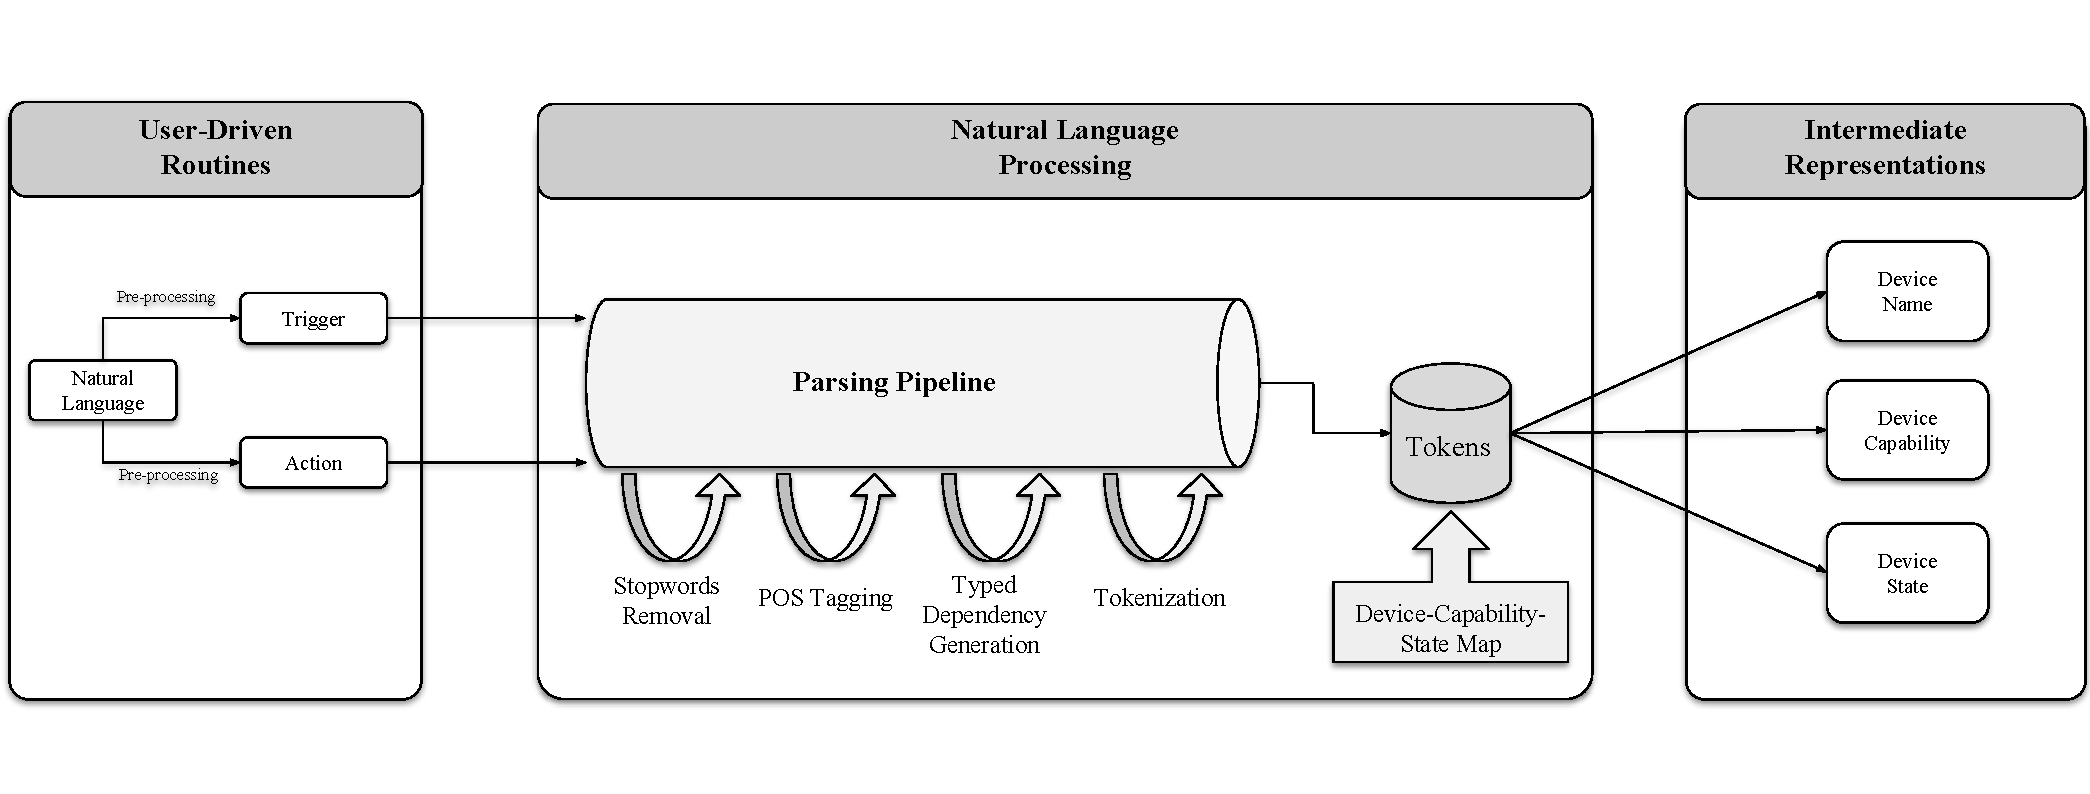
\includegraphics[width=\textwidth]{figs/nlp-tool-final.pdf}
    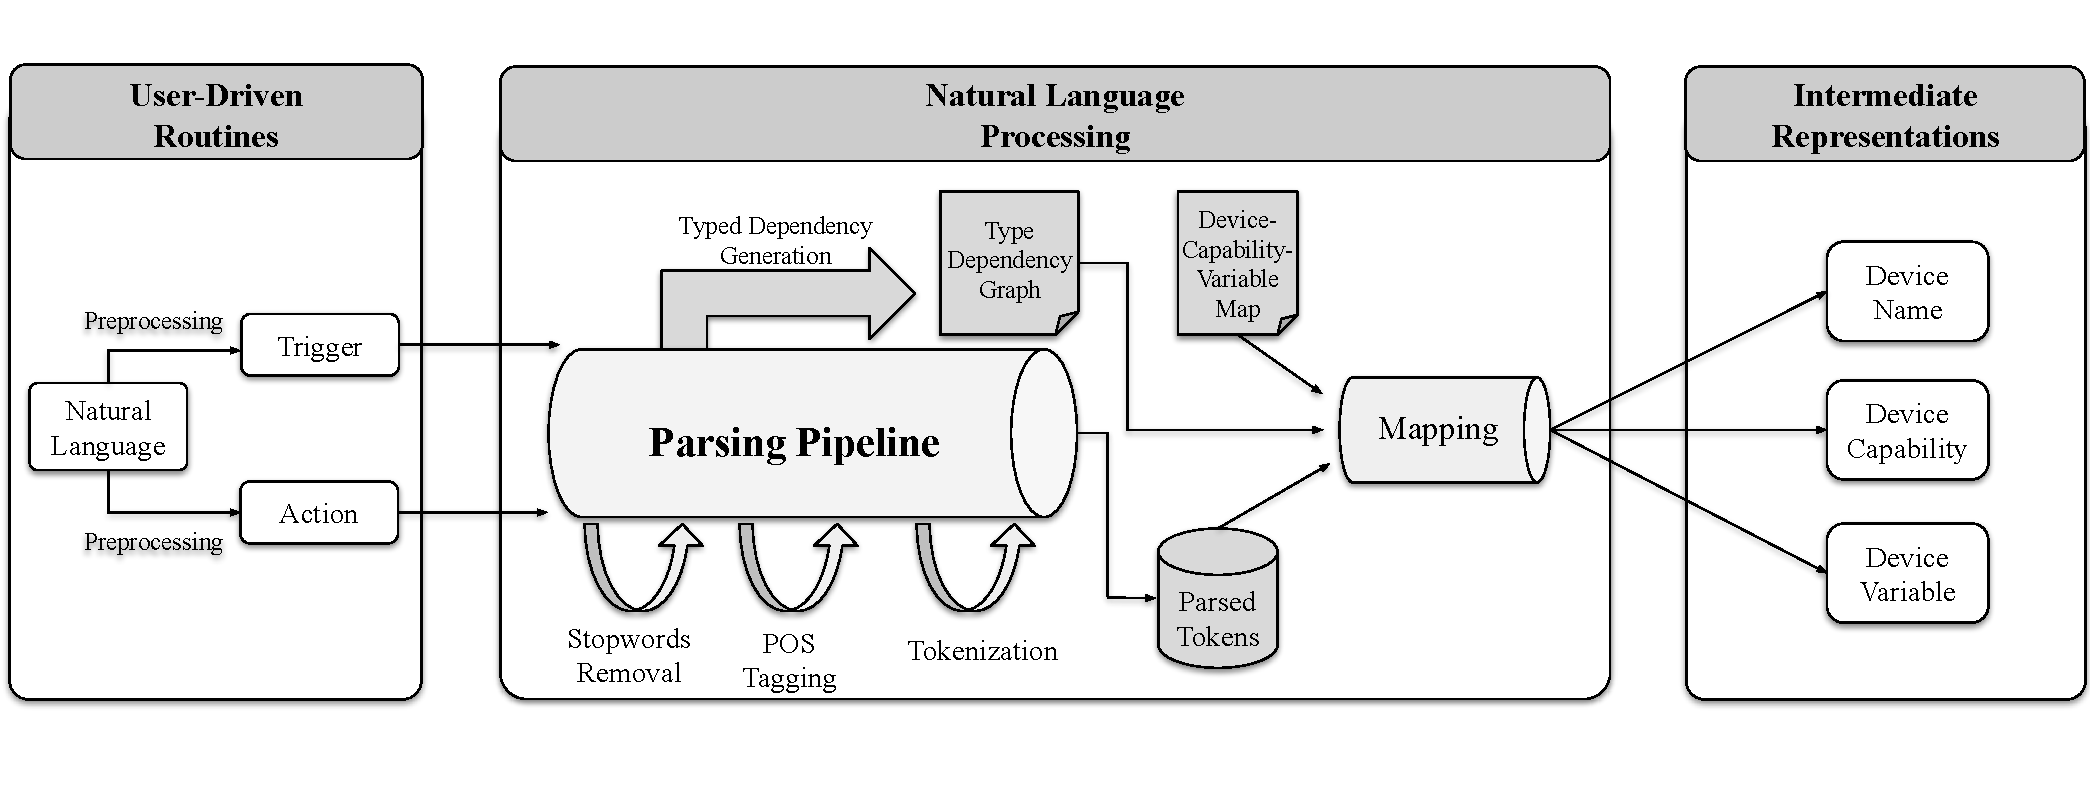
\includegraphics[width=\textwidth]{figs/nlp-tool-final-v2.pdf}
    \caption{Overview of the framework for transforming user-driven routines into intermediate representation (IR)}
    \label{fig:nlp-framework}
\end{figure*}




In this section, we will describe our design choices of our approach of transforming user-driven routine to intermediate representation. Figure.~\ref{fig:nlp-framework} provides an overview of the three main stages.


\subsection{Design choices}
One of the other main goals of this project is to be able to generate intermediate representation \textit{automatically}. In order to automate the process of converting user written routines to execution indicators for systematic testing, we use NLP techniques to extract devices information from human written routines. We extract and
correlate the behaviors in three layers: {\sf (1)} device name, {\sf (2)} device capability, and {\sf (3)} device variable (state).

As mentioned before, this approach consists of three main steps. In Step 1, we \textit{pre-processes} user-driven routines through splitting them by ``If'' and ``Then'', these syntactic indicators were provided for participants when creating routines. Since both the trigger and action should each contain all the device information needed to generate the intermediate representation, we could treat them as the same problem and pass them into the same program following the same procedure.

Although triggers and actions might seem to be distinct at first glance, they share sufficient amount of similarity that can be consider equivalent in terms of being considered as input to our models (one for each intermediate representation type).

We can list the similarities as the follows:
\begin{itemize}
    \item \textbf{Similarity 1:} Triggers and actions both have to specify the three characteristics of the devices in one way or another. For example: If air temperature is greater than 80, turn on the air conditioner. Both trigger and action have to specify some characteristic about the device.
    \item \textbf{Similarity 2:} Trigger are often expressed as an action, and the reverse is also true. For example, ``turn on the light'' can act both as the trigger of one routine and as the action of another. This demonstrates that there is not much difference in the essence of the phrase.
\end{itemize}
% Proof that trigger and action are the same

One other design decision we made is that we required participants of the survey to use conjunction ``AND'' or ``OR'' in all capitalized characters when combining the different trigger conditions. This is to help our models to recognize each distinct trigger condition more accurately without imposing much constraint on user. 

Some triggers, such as Location Mode and Time, does not have a physical device associated with them. In those cases, we create a new device type called ``Null'' with the respective capabilities to incorporate them. By doing so, we were able to prevent ourselves to omit some virtual trigger conditions.

Following the pre-processing procedure in the above manner, we can obtain a list of triggers conditions and a list of actions. For the proof of concept, we implement this approach on the list of triggers. Applying this method to the list of actions is trivial, all we have to do is to replace the input from trigger conditions to the action phrases.

The processed triggers will then be pass into the next stage, the Parsing Pipeline, where the major part of the Natural Language Processing takes place. After trying out different part of speech taggers, we settled with Stanford CoreNLP POS Tagger~\cite{Manning2014} as it was able to perform better than the default NLTK POS Tagger.

The result of the Parsing Pipeline, combine with the addition of the device-capability-variable map and type dependency graph, will then be mapped into the resulting three intermediate representation.



\subsection{Preprocessor}

Our pre-processor accepts plain English text as the input and reduces the number of lexical tokens by eliminating unnecessary words and unrecognizable characters or words. In particular, the preprocessor performs the following pre-processing tasks:
\begin{itemize}
    \item \textbf{Comparison Handling: } Many routines contain value comparisons as their trigger conditions. However, since there is no constraint to what user can input, we observed that a substantial number of participants uses comparison operators (\eg ``>'', ``<'', etc) to construct their routines. Therefore, in order to have NLP tools to recognize these important symbols, We replaces all instances of comparison operators into English plain text. 
    \item \textbf{Stop words removal: } We follow standard NLP practices to pre-process our data, such as removing stop words (\eg ``a'', ``this'', ``the'') using NLTK library. 
    \item \textbf{Whitelisting input: } Since there is no enforcement in our user input, we whitelisted the routines using regular expression filtering. We only accepted a narrow set of input such as characters and numbers, and punctuation symbols as these sentences would become our input to the NLP parser.
\end{itemize}


\subsection{NLP Parser}
Our NLP Parser accepts the pre-processed sentences and annotates each words within a sentence using standard NLP techniques. We perform the following tasks with the Stanford CoreNLP parser:
\begin{itemize}
    \item \textbf{Name Entity Recognition: } We use the parser to identify named entities (\eg person names, organizations) in each routine. In addition, these entities are added to a dictionary so that we can perform additional natural language processing.
    \item \textbf{Part of Speech Tagging: }  We use Stanford POS Tagger to process each word in a given routine. We see that often the case that nouns are more related to the device name than the others; for example, ``smoke'' is good indicator of a ``smoke detector''.  While most cases are more complex than this example, we used this as one of our indicator for selecting the possible candidate for intermediate representation of Device Name. Similar approach can be used on identifying possible words that represents the Device Variables such as ``on'' or ``off'', which corresponds to part of speech ``IN'', preposition/subordinating conjunction. As for device capability, we noticed that they are generally associated with ``VB'', verb (\eg lock the door), would be mapped to door.lock.
    \item \textbf{Typed Dependency Generation: } Our more comprehensive analysis follows. Specifically, we use Stanford parser to annotate each routine with Stanford-typed dependency. One sample typed dependency graph generation of trigger condition is shown by Figure.~\ref{fig:dep-tree}. These information can be used later to help generating the intermediate representation mapping.
    \item \textbf{Tokenization: } When performing the above techniques, Stanford Parser would automatically tokenize each word in the sentence and output them as a tuple. This is important during the mapping phase since it saves the result of POS and type dependency generation with the associated word.
\end{itemize}

\subsection{Intermediate Representation Mapping}

From the result of the Parsing Pipeline, we were able to get a list of parsed tokens with valuable syntactic information associated with them. In order to create the three different types of intermediate representation, we would need to perform the mapping in three distinct ways. Before making different models, we created a device-capability-variable mapping with the all the devices mapped with its capabilities and with the possible variables / states that it can take. This mapping was done separately from the user-driven routines since it does not require any information from end-users. In order to create a model that can generate the desired intermediate representation, we would look at each token in a given routine, and examine its part of speech in addition to its typed dependency, and finally check for the device-capability-variable map as a way of confirmation.


\begin{figure}[t]
    %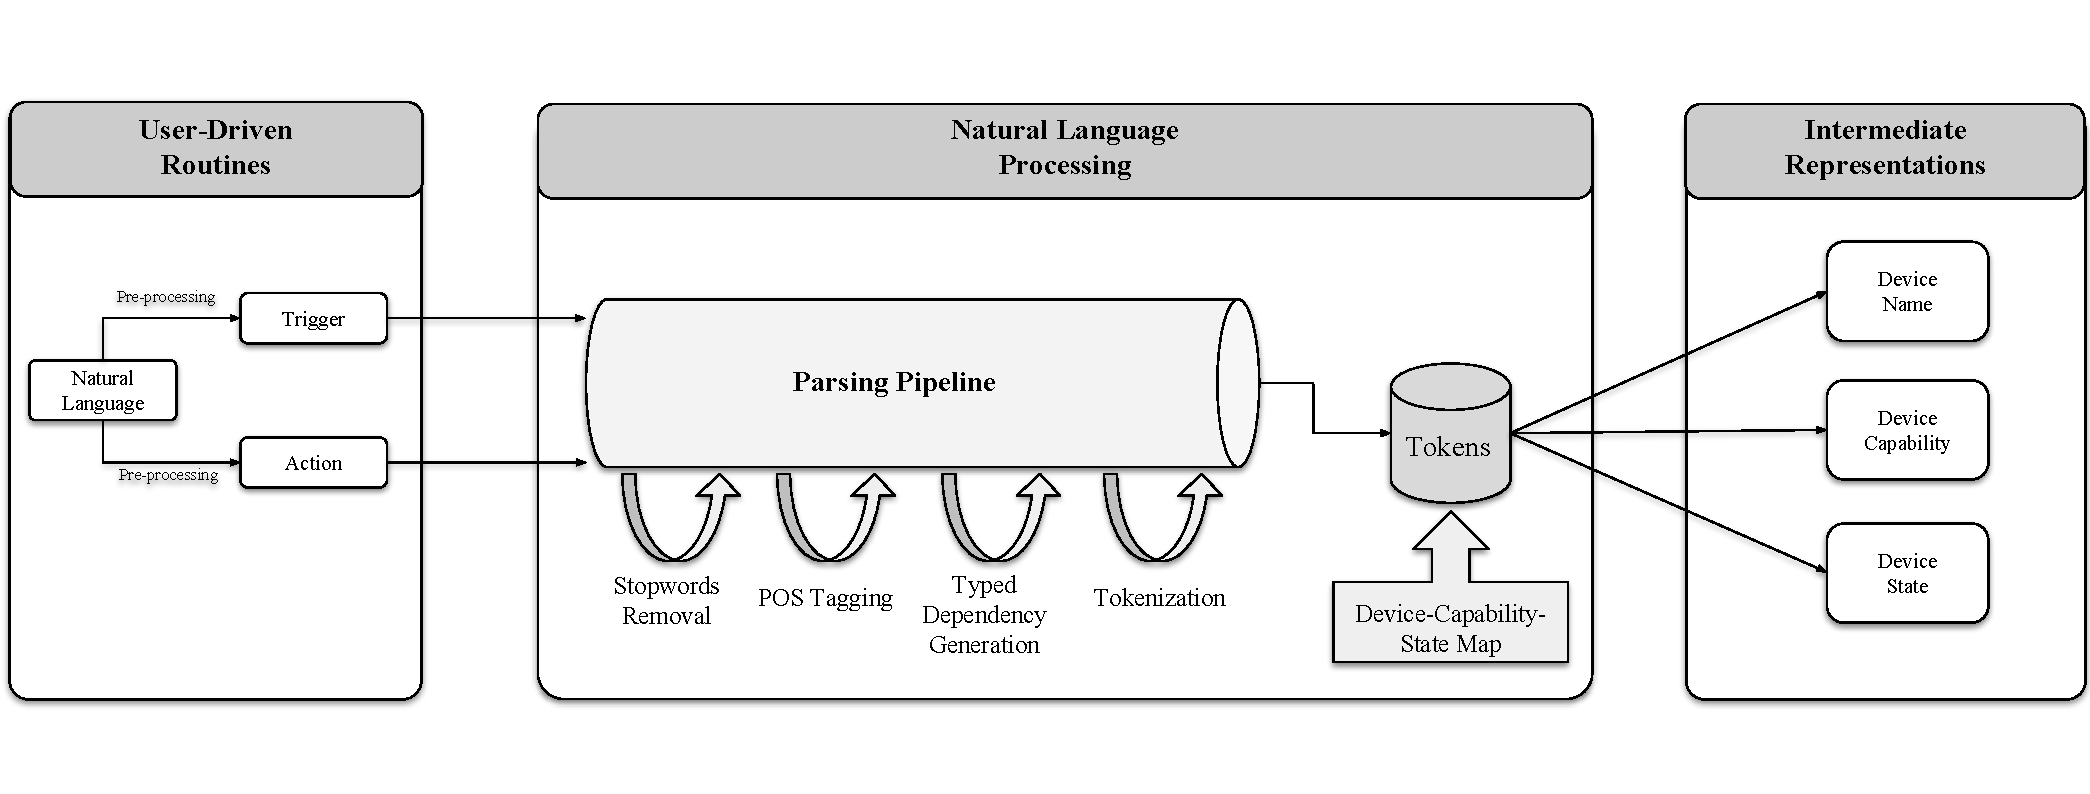
\includegraphics[width=\textwidth]{figs/nlp-tool-final.pdf}
    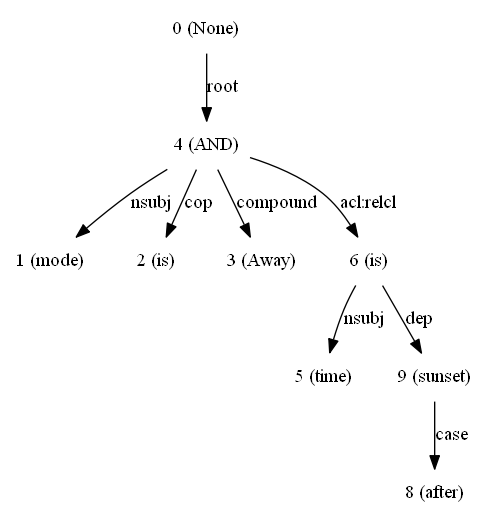
\includegraphics[width=3.5in]{figs/dep_good.png}
    \caption{Typed Dependency Graph of a Sample User-Driven Trigger}
    \label{fig:dep-tree}
\end{figure}





%
\section{Implementation}
\label{sec:implementation}

This section provides the implementation detail of the intermediate representation generation framework. Our framework consists of three stages: a pre-processor, a NLP parser, and an intermediate representation generator. The pre-processor accepts list of trigger conditions or action phrases as input and preprocesses them for the NLP parser. The intermediate representation generator accepts the pre-processed phrases and parse them using the NLP parser.


%$$p(c|w;\theta) = \frac{e^{v_c \cdot v_w}}{\sum_{c^\prime\in C}e^{c^\prime \cdot v_w}}$$
%$$p(c|w;\theta) = \frac{e^{v_c*v_w}}{\sum_{c \in C}e^c'*v_w}$$






\section{Evaluation}
\label{sec:eval}

% \textbf{Evaluation (don't forget to interpret your data)}

%In order to determine the accuracy of our models prediciting the 

The main goal of our evaluation is to measure the effectiveness of our models at extracting and transform key device characteristics into their respective intermediate representations. For this study, we focus on evaluating against the existing dataset of 250 user-driven routines.
To test for the accuracy of the models we generated, We first manually went over each routine and produce the intermediate representations. Then, we compare the result of our manual effort with the intermediate representations generated by our models. In the end, our models were able to extract device name, device capability, and device variables with an accuracy of 80.64\%, 58.04\%, and 64.29\% respectively. We were able to extract device name with the highest accuracy because device name often exist as is in the natural text from end-user, and we were able to extract them with minimum effort. This approach is still limited in the sense that it cannot contents that are not inside the given input. This is probably the reason that we are unable to have a decent accuracy fro device capability, which are often are not explicit.


\section{Additional Insights}
\label{sec:insight} 

% Give stats on survey (i.e., users, experience, etc.)
%We used the survey methodology briefly described previously (and in detail in Appendix~\ref{app:survey_methodology} to collect routines, execution indicators, and additional information from 37 users, after discarding \xy surveys with random/incomplete responses.
%population

%While the prior sections examine how \tool can be used to analyze the naturalness/security flaws of home automation, 

While the prior sections focused on the design and implementation of the generation of intermediate representation approach, this section describes several insights that can be drawn from the result of this approach with answers to a sereies of research qeustions (\textbf{RQ}). In order to get a more accurate grasp of the results, we use the manually generated intermediate representation.

\myparagraph{RQ 1   - How diverse is our dataset, \ie how many unique routines?}

One of the core features of the intermediate representation is its ability to abstract and characterize the given user-driven routine. We know that a routine consists if triggers and actions. We can  define a routine to be``unique'' if it is consisted of different combinations of intermediate representation. In other words, if two routines end up having the same trigger and action intermediate representations, they are considered equivalent. By using this approach, we created a dictionary that maps each routine with an aggregation of all of its intermediate representations. For example, an simple routine:   
\noindent\fbox{%
    \parbox{\linewidth}{%
    If it is morning, then turn on the Coffee Maker.
	}
}
would have the following aggregation: 
\noindent\fbox{%
    \parbox{\linewidth}{%
    'Morning + switch + on + Coffee Maker + switch + on'
	}
}

To count the total number of unique routine, we simply count the number of unique aggregations of intermediate representation. In the end, we found that there are \textbf{220} unique user-driven routines, or 88\%, in the dataset of 250. The approach we used is a overestimation that serve as the higher bound of measuring number of unique routines. An alternative method to perform the aggregation of intermediate representation is to only include the device names and device capabilities, without device variables. Intuition behind this is that device variables represents the state or the condition for the device's capability, as which does not offer much difference to a similar routine that uses the same device and capability. 


\myparagraph{RQ 2   - Top 8 most common routines} 

\begin{table}[t]
\centering
\scriptsize
\caption{{\small Top 8 most common routines}}
\label{tbl:top-8-routines}
\begin{tabular}{c|c}
\Xhline{2\arrayrulewidth}
{\bf Routine}& {\bf Count}\\
\Xhline{2\arrayrulewidth}
 Turn Off/On the Air Purifier based on air quality. & 6 \\
 Change the Thermostat mode based on room temperature. & 5 \\
 Change the AC mode based on the room temperature. & 5 \\
 Change the AC mode based on the mode of the home. & 4 \\
 Open/close the window Shades/Blinds based on the time. & 4 \\
 Turn on the CoffeeMaker based on time of the day. & 4 \\
 Sound the security alarm if smoke is detected. & 3 \\
 Lock the door at Night. & 3 \\
\Xhline{2\arrayrulewidth}
\Xhline{2\arrayrulewidth}
\end{tabular}
\end{table}

Using similar strategy as before, we create a mapping of the aggregated intermediate representation of each routine and a count variables. After iterate though the entire dataset, we present the most common routine that is used in our dataset as shown in Table.~\ref{tbl:top-8-routines}. It is quite interesting to observe that Air quality and temperature are the most common factor that the user most wanted to control. This result is helpful to for critical stakeholders such as platform vendors, end-users, and security researchers to prioritize analysis related to temperature control.

\myparagraph{RQ 3   - What are the most common devices used by users?}

\begin{table}[t]
\centering
\scriptsize
\caption{{\small Top 8 devices user want}}
\label{tbl:top-8-devices}
\begin{tabular}{c|c|c}
\Xhline{2\arrayrulewidth}
{\bf Device Name}& {\bf Count}& {\bf \%}\\
\Xhline{2\arrayrulewidth}
Air Conditioner & 32 & 86.49\\
Light Bulb & 32 & 86.49\\
Thermostat & 28 & 75.68\\
Security Camera & 27 & 72.97\\
Security Alarm & 26 & 70.27\\
Door Lock & 25 & 67.57\\
Audio Player & 23 & 62.16\\
Temperature Sensor & 23 & 62.16\\
\Xhline{2\arrayrulewidth}
\Xhline{2\arrayrulewidth}
\end{tabular}
\end{table}

To get an insight on the devices being used by user, we look at the device name for each routine (both trigger and action) and increment the count once for each device being used by each user (we did not count multiple instances of the same device used by one user), as shown in Table.~\ref{tbl:top-8-devices}. This result is also interesting as it shows that, once again, user prefer to incorporate Air Conditioner(over 85\%) / Thermostat control in their home automation, supporting the previous finding in \textbf{RQ 2}.

\myparagraph{RQ 4   - What are the most common trigger conditions?} 

\begin{table}[t]
\centering
\scriptsize
\caption{{\small Top 8 trigger conditions}}
\label{tbl:top-8-trigger}
\begin{tabular}{c|c|c}
\Xhline{2\arrayrulewidth}
{\bf Trigger}& {\bf Count} &{\bf \%}\\
\Xhline{2\arrayrulewidth}
locationMode+Null & 27 & 72.97\\
switch+Morning & 14 & 37.84\\
presence+Presence Sensor & 13 & 35.14 \\
switch+Night & 12 & 32.43\\
temperature+Temperature Sensor & 12 & 32.43\\
temperature+Thermostat & 8 & 21.62\\
motion+Motion Sensor & 7 & 18.91\\
airQuality+Air Purifier & 6 & 12.77\\
\Xhline{2\arrayrulewidth}
\Xhline{2\arrayrulewidth}
\end{tabular}
\end{table}

We collect the number of triggers (aggregated device name and device capability of the intermediate representation), and we found out that most user (over 70\%) would utilize ``Mode'' as the trigger for their automation, as shown in Table.~\ref{tbl:top-8-trigger}

\myparagraph{RQ 5   - What are the most common actions?} 

\begin{table}[t]
\centering
\scriptsize
\caption{{\small Top 8 actions}}
\label{tbl:top-8-action}
\begin{tabular}{c|c|c}
\Xhline{2\arrayrulewidth}
{\bf Action}& {\bf Count}&{\bf \%}\\
\Xhline{2\arrayrulewidth}
thermostat+Air Conditioner & 28 & 75.68\\
switch+Light Bulb & 20 & 54.05\\
alarm+Security Alarm & 16 & 43.24\\
notification+Phone & 12 & 32.43\\
lock+Door Lock & 11 & 29.73\\
contact+Shades/Blinds & 10 & 27.02\\
switch+Security Camera & 9 & 24.32\\
thermostat+Thermostat & 8 & 21.62\\
\Xhline{2\arrayrulewidth}
\Xhline{2\arrayrulewidth}
\end{tabular}
\end{table}

Similar as the approach to \textbf{RQ 4}, we total the number of unique actions, based on the device name and device capability. And found out that Aic Conditioner is the most popular (over 75\%) action to perform, as shown in Table.~\ref{tbl:top-8-action}


\myparagraph{RQ 6   - Can existing IoT marketplace apps satisfied most end-users' requirement? } 

\begin{table*}[t]
\centering
\scriptsize
\caption{{\small Analysis of Public SmartThings Repo}}
\label{tbl:public-analysis}
\begin{tabular*}{\textwidth}{c|c|c}
\Xhline{2\arrayrulewidth}
{\bf Method}&{\bf }& {\bf Count}\\
\Xhline{2\arrayrulewidth}
\rule{0pt}{3ex} \multirow{2}{*}{Manual}  & RAW routines that can be represented with one of the public smart apps & 143 \\
& RAW routines that \textbf{CANNOT} be represented with one of the public smart apps & 107 \\
\Xhline{2\arrayrulewidth}
\Xhline{2\arrayrulewidth}
\rule{0pt}{3ex} \multirow{2}{*}{Device Name + Device Capability} & Unique routines that can be represented with one of the public smart apps & 99 \\
& Unique routines that \textbf{CANNOT} be represented with one of the public smart apps & 90 \\
\Xhline{2\arrayrulewidth}
\Xhline{2\arrayrulewidth}
\rule{0pt}{3ex} \multirow{2}{*}{Device Name + Device Capability + Device Variable} & Unique routines that can be represented with one of the public smart apps & 124 \\
& Unique routines that \textbf{CANNOT} be represented with one of the public smart apps & 97 \\
\Xhline{2\arrayrulewidth}

\end{tabular*}
\end{table*}


One of our core arguments for a paradigm shift from the predominant trend of analyzing marketplace IoT apps is that marketplace IoT apps are constrained by the limited perspective of third-party developers. Often times, end-users' direct requirement are not satisfied. Therefore, a key research question we ask is that can existing IoT marketplace apps satisfied most end-users' requirement? 
We conducted three experiments to assess our arguments. We first went over each routine using intermediate representation as a guide and manually determined whether if an existing IoT app can satisfy the end-user's requirements, we refer this as the ``Manual'' method. The manual method demonstrates that 107 out of 250, 42.8\%, of the user-driven routines cannot be represented with one of public smart apps from SmartThings. Since many user-driven routines are similar and might effect the ratio, we filter the result based on two method, one focus on Device Name and Device Capability, with 47.62\% cannot be represented by public IoT apps, while the other focus on all three intermediate representations, with 43.89\% cannot be represented (Table.~\ref{tbl:public-analysis}). For all three cases, there are more than 40\% of user-driven routines that cannot be represented with one of public smart apps from SmartThings. This further calls for a paradigm shift from the traditional focus of solely on marketplace IoT apps.




%These results also reinforce the validity of \tools informed execution that makes use of these execution indicators.

%More importantly, they are ``unsure'' in very few cases (\ie\ {\em at most 18.4\% for frequency}).  
%On further examining the data, we discover that most of these unsure cases are caused by unpredictable triggers, such as CO leaks, smoke, and drastic temperature changes, which is understandable. 
%More importantly, our survey clearly demonstrates that users are able to confidently predict a significant number of execution indicators, although some triggers may make this difficult.
%%%%%%%%%%%%%%%

%%% Interesting insights



%%%

% 3. What devices do users want in their homes? 
%% light bulb 32,  ac 31, thermostat 28, sec camera 27, sec alarm 26, door lock 25, temperature sensor 23, smart audio player 22,  smart TV + Smart Speaker + Smoke Detector 21, garage door opener 20, 

% 4. Push-Notified when routines are triggered  :
%% Always (6 or 16), Very frequently (7 or 18), Occasionally (14 or 37), Rarely (6 or 16), Never (4 or 10)


%% 5. Consider security when creating routines? VERIFY 
% Always 17, Most of the time 14, 3 rarely or never (2+1)

% 6. Trust routines by 3party devs: VERIFY
%% sometimes (21), most of the time (6), rarely (7), never (4), always 0

%7. Would you test your routines to make sure they execute as you want them to? VERIFY
%% always 21, almost always 11, occasionally 5, never 1
 
%%%%%%%%%%%%%%%%
%%% Results to support the design

% 11. Execution indicators
%% 11.a) Time of day: not sure (6) mostly for air quality bad, motion or glass break detected, water leak or CO or smoke detected, temperature changes, certain (147), anytime (97)
%% 11.b) Frequency: not sure (46), more factors (e.g., security camera takes picture, water leak, odorLevel of Gas Sensors), certain (204)
%% 11.c) Weekday/Weekend: Not sure (21), throughout the week (171), weekday/weekend (57)


\section{Discussion}
\label{sec:discussion}

In addition to perform POS tagging, we could try to group words that are similar to each other by encode each word to numerical vectors representation. This can be achieved using Word2Vec, a state-of-art tool that used to produce word embedding. Word2Vec is a group of models, Specifically, two-layer neural networks that are trained to reconstruct linguistic contexts of words. It takes a corpus as input and produces a vector space, with each unique words in the corpus assigned with a corresponding vectors.
Word2Vec was created by a group of researchers at Google led by Tomas Mikolov. Some advantages of Word2Vec over other rival tool such as WordNet is that it can better capture syntactic and semantic information and it can achieve a lower false positive rate than ESA (Explicit Semantic Analysis)  Word2Vec also offer two types of model to produce representation of word: Continuous bag-of-word (CBOW) or continuous skip-gram. In CBOW model, the model predicts a word from a range of surrounding words. On the other hand, a skip-gram model uses the current word to predict the surrounding windows of context words. This model is able to achieve this by assigning more weight to the neighboring words than more distant words.
This technique will be useful in that we will be able to group device with its capabilities and states, and this will have a more predicting power than a standard POS tagging approach.
We were unable to perform this techniques due to a limited number of data to train the model, but can be used for future work.

\section{Related Work}
\label{sec:related-work}
In terms of leveraging NLP tools to perform analysis of the security of smart home automation, work by Tian et al. (SmartAuth)~\cite{tzl+17} and Ding et al. (IoTMon)~\cite{dh18} are similar to our paper. However, there are some key differences. First, we target different region of the home automation system. While both Tian and IoTmon are using NLP techniques to analyze IoT application, routines created by third-party developers, descriptions to identify physical channel in IoT platform, our goal is leveraging NLP techniques to analyze the \textit{user-driven} routines. Second, we utilize the result of NLP for a different purpose. While they integrated NLP techniques to devise static analysis system to detect different security violations, we leverage NLP techniques for a quantitative analysis, and call for a motivation to prioritize routines that are used more common by real users. In addition, we investigated and propose a method that enables the analysis of user-driven routines, which are less common research area.
The closest relevant work is by Surbatovich et al.~\cite{sab+17}. They also focused on the idea of the need to examine \textbf{both} user created and developer-created If-This-Then-That (IFTTT) recipes, analogous to what an IoT app is. However, we differ in the problem scope and domain. IFTTT is a platform that connects external services like Instagram or Twitter to smart home devices. For example, user can create an IFTTT recipe that can turn on a smart light when the pizza delivery guy is on his way. This work by Surbatovich et al. focuses on exposing security and privacy ramifications of IFTTT recipes. In contrast, our goal is to enable analysis of user-driven routine in home automation, which limits our scope to events within users' home.

%sequences composed from multiple routines.


%Prior work has proposed a diverse set of security systems and analyses for smart homes. 
%In terms of analysis and enforcement, the natural perspective provided by \tool is complementary to the diverse set of security systems and analyses for smart homes proposed by prior work.
%For instance, consider ContexIoT~\cite{jcw+17}, an access control system that prompts the user for authorization whenever it identifies the use of sensitive operations (\eg unlocking the door) in new contexts.
%To measure the frequency of user-prompts (\ie which affect usability), ContexIoT uses random event sequences generated by fuzz testing of IoT apps.
%The test cases predicted by \tool would provide a more realistic input, 
%%relative to random event sequences, 
%leading to a representative evaluation for such systems.
%Similarly, IoTSAN~\cite{nsq+18}, a system that uses model checking to analyze IoT setups for safety, also uses random events for evaluation, and may similarly benefit from \tool. 
%Additionally, \tools\ {\em down} flavor can directly contribute to adversarial benchmarks such as IoTBench~\cite{cmt18}, for effective evaluation of future work.
%
%Finally, policy-based enforcement for the smart home (\eg ProvThings~\cite{whbg18} and IoTGuard~\cite{ctm19}) can significantly benefit from \tools semi-automated approach for creating policies (Sec.~\ref{sec:security_researchers}).
%For instance, ProvThings~\cite{whbg18} is a provenance tracker for the SmartThings platform, which can also enforce policies. 
%However, it relies on manually-curated policies that are generated from already-occurred security incidents, or domain expertise. 
%As described in Section~\ref{sec:case_studies}, \tool can help security experts create effective policies arising from natural regularities in user-driven home automation sequences, without significant manual effort.
%Analysis that relies on security or safety policies, such as Soteria~\cite{cmt18} and IoTSan~\cite{nsq+18}, can similarly benefit from \tool. 

%\myparagraph{2. Treating software as a natural language} 

\section{Conclusion}
\label{sec:conc}

In this paper, we demonstrated and motivated the need for a way to enable then analysis of user-driven routines. We presented a systematic approach of extracting device names, device capabilities, and device state / condition using a combination of state-of-art NLP tools and techniques. We evaluated this approach with the manually labeled result of 250 routines from our user study. The result demonstrated that we were mostly successful in extracting device name from the natural language routines with a 80\% accuracy. However, due to the fact that device capabilities and device condition / states are vague and often represented as complex phases, our straightforward approach were less accurate in extracting the corresponding device capabilities and device conditions. In future work, we can improve this kind of extraction with and  potentially with another layer of extraction so that we can generate more accurate models, thus making generation of intermediate representation more representative when converting to IoT smart apps for further platform-wise testing. 



%-------------------------------------------------------------------------------




%-------------------------------------------------------------------------------
\section*{Acknowledgments}
I would like to express my sincere gratitude to my honors adviser, Professor Adwait Nadkarni, for his continuous support during my project. I would also like to thank Sunil Manandhar for his continuous support and valuable feedback during time of doubt. Lastly, I am grateful to my friends for their patience and encouragement that fueled me throughout the year.
%-------------------------------------------------------------------------------



\bibliographystyle{plain}
\bibliography{bibliographies/os,bibliographies/semeru,bibliographies/iot,bibliographies/misc,bibliographies/phone,bibliographies/monkeylab}



%-------------------------------------------------------------------------------
\end{document}
%-------------------------------------------------------------------------------


